%%%%%%%%%%%%%%%%%%%%%%%%%%%%%%%%%%%%%%%%%
% a0poster Landscape Poster
% LaTeX Template
% Version 1.0 (22/06/13)
%
% The a0poster class was created by:
% Gerlinde Kettl and Matthias Weiser (tex@kettl.de)
% 
% This template has been downloaded from:
% http://www.LaTeXTemplates.com
%
% License:
% CC BY-NC-SA 3.0 (http://creativecommons.org/licenses/by-nc-sa/3.0/)
%
%%%%%%%%%%%%%%%%%%%%%%%%%%%%%%%%%%%%%%%%%

%----------------------------------------------------------------------------------------
%	PACKAGES AND OTHER DOCUMENT CONFIGURATIONS
%----------------------------------------------------------------------------------------

\documentclass[a0,portrait]{a0poster}

\usepackage{multicol} % This is so we can have multiple columns of text side-by-side
\columnsep=100pt % This is the amount of white space between the columns in the poster
\columnseprule=3pt % This is the thickness of the black line between the columns in the poster

\usepackage[svgnames]{xcolor} % Specify colors by their 'svgnames', for a full list of all colors available see here: http://www.latextemplates.com/svgnames-colors

\usepackage{times} % Use the times font
%\usepackage{palatino} % Uncomment to use the Palatino font

\usepackage{graphicx} % Required for including images
\graphicspath{{figures/}} % Location of the graphics files
\usepackage{booktabs} % Top and bottom rules for table
\usepackage[font=small,labelfont=bf]{caption} % Required for specifying captions to tables and figures
\usepackage{amsfonts, amsmath, amsthm, amssymb} % For math fonts, symbols and environments
\usepackage{wrapfig} % Allows wrapping text around tables and figures

\usepackage{tikz}
\usepackage{subfigure}


\usepackage{textcomp} % \textdegree

\begin{document}

%----------------------------------------------------------------------------------------
%	POSTER HEADER 
%----------------------------------------------------------------------------------------

% The header is divided into three boxes:
% The first is 55% wide and houses the title, subtitle, names and university/organization
% The second is 25% wide and houses contact information
% The third is 19% wide and houses a logo for your university/organization or a photo of you
% The widths of these boxes can be easily edited to accommodate your content as you see fit

\begin{minipage}[b]{0.8\linewidth}
\veryHuge \color{NavyBlue} \textbf{Diabetic Retinopathy Detection through Image Analysis Using Deep Convolutional Neural Networks} \color{Black}\\ % Title
%\Huge\textit{An Exploration of Complexity}\\[1cm] % Subtitle
\huge \textbf{Jordi de la Torre, Aida Valls \& Domenec Puig}\\ % Author(s)
\huge Departament d'Enginyeria Inform\`atica i Matem\`atiques\\
\huge Universitat Rovira i Virgili\\ % University/organization
%\end{minipage}
%
%\begin{minipage}[b]{0.25\linewidth}
\color{DarkSlateGray}\Large \textbf{Contact Information:}\\
Email:\\ 
\texttt{jordi.delatorre@gmail.com}\\ % Email address
\texttt{aida.valls@urv.cat}\\
\texttt{domenec.puig@urv.cat}\\
\end{minipage}
%
\begin{minipage}[b]{0.19\linewidth}

\includegraphics[width=20cm]{logourv.eps} % Logo or a photo of you, adjust its dimensions here
\end{minipage}

\vspace{1cm} % A bit of extra whitespace between the header and poster content

%----------------------------------------------------------------------------------------

\begin{multicols}{3} % This is how many columns your poster will be broken into, a poster with many figures may benefit from less columns whereas a text-heavy poster benefits from more

%----------------------------------------------------------------------------------------
%	ABSTRACT
%----------------------------------------------------------------------------------------

\color{Navy} % Navy color for the abstract

\begin{abstract}

Diabetic Retinopathy is one of the main causes of blindness and visual impairment for diabetic population. The detection and diagnosis of the disease is usually done with the help of retinal images taken with a mydriatric camera. In this paper we propose an automatic retina image classifier that using supervised deep learning techniques is able to classify retinal images in five standard levels of severity. In each level different irregularities appear on the image, due to micro-aneurisms, hemorrages, exudates and edemas. This problem has been approached before using traditional computer vision techniques based on manual feature extraction. Differently, we explore the use of the recent machine learning approach of deep convolutional neural networks, which has given good results in other image classification problems. From a training dataset of around 35.000 human expert classified images, different convolutional neural networks with different input size images are tested in order to find the model that performs the best over a test set of around 53000 images. Results show that it is possible to achieve a quadratic weighted kappa classification score over 0.75 not far from human expert reported scores of 0.80.

\end{abstract}

%----------------------------------------------------------------------------------------
%	INTRODUCTION
%----------------------------------------------------------------------------------------

\color{SaddleBrown} % SaddleBrown color for the introduction

\section*{Introduction}

Diabetic Retinopathy (DR) is a leading disabling chronic disease  and  one of the main causes of blindness and visual impairment in developed countries for diabetic patients. Studies reported that 90\% of the cases can be prevented through early detection and treatment \cite{torrents15}. Eye screening through retinal images is used by physicians to detect the lesions related with this disease. 

The DR disease is standardly classified \cite{diaclass} in the next fixe classes:

\begin{enumerate}
	\item [0.]\setcounter{enumi}{0} - No apparent retinopathy
	\item - Mild Non-Proliferative Diabetic Retinopathy (NPDR)
	\item - Moderate NPDR
	\item - Severe NPDR
	\item - Proliferative DR
\end{enumerate}

In this paper we propose an automated classification of retinal images into these 4 classes using Deep Learning techniques. 

\begin{center}
	\captionof{figure}{Image samples of the five different DR severity classes sorted from 0 (left) to 4 (right)}
	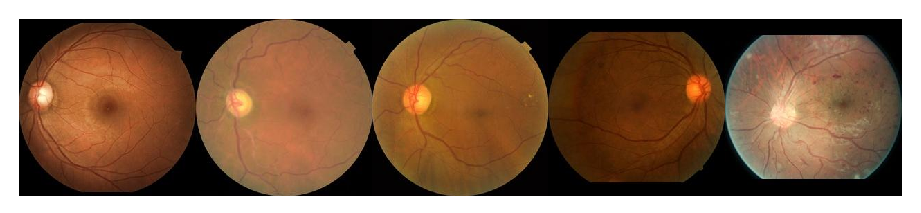
\includegraphics[width=20cm]{5classes.eps}
	\label{image-classes}
\end{center}


\color{DarkSlateGray} % DarkSlateGray color for the rest of the content

%----------------------------------------------------------------------------------------
%	MATERIALS AND METHODS
%----------------------------------------------------------------------------------------

\section*{Methodology}

\subsection*{Evaluation function}

The performance of the classification model is measured using the quadratic weighted kappa  (QWK) index. See equation \ref{eq:kappa}. 

\begin{equation}\label{eq:kappa}
\kappa = 1 - \frac{ \sum_{i=1}^C \sum_{j=1}^C \omega_{i,j} O_{i,j} }
{\sum_{i=1}^C \sum_{j=1}^C  \omega_{i,j} E_{i,j}}
\quad \textrm{where} \quad \omega_{i,j} = \frac{(i-j)^2}{(C - 1)^2}
\end{equation}

The interpretation of kappa values can be done using the guide of table \ref{kappa-interpretation}.

\begin{center}
	\captionof{table}{Table Interpretation of kappa, after Landis and Koch (1977)}
	\begin{tabular}{llr}
		\hline
		Kappa    & Strength of agreement \\
		\hline
	    \textless 0.20 		& Poor \\
		0.21-0.40 	& Fair \\
		0.41-0.60 	& Moderate \\
		0.61-0.80 	& Good \\
		0.81-1.00 	& Very good \\
		\hline
	\end{tabular}
	\label{kappa-interpretation}
\end{center}

\subsection*{The Data}

The training set contains a total of 35.126 high resolution images; 25.810 of class 0, 2.443 of class 1, 5.292 of class 3, 873 of class 3 and 708 of class 4. The test set contains a total of 53.576 high resolution images; 39.533 of class 0, 3.762 of class 1, 7.861 of class 2, 1.214 of class 3 and 1.206 of class 4. Notice that it is highly imbalanced. 

All the images are classified by ophthalmologists according to the standard severity scale presented before \cite{diaclass}.

From the training data we can extract the frequency of combined occurrence of the disease in both eyes of the same patient. Table \ref{table-frequencies} show this frequencies.

\begin{center}
	\captionof{table}{Frequencies of combined occurrence of classes (left eye: rows, right eye: columns)}	
	\begin{tabular}{c c c c c c c} 
		\hline
		Eyes & C0 & C1 & C2 & C3 & C4 & Sum\\ [0.5ex] 
		\hline\hline
		C0 & 12155 & 407 & 295 & 3 & 11 & 12871\\
		C1 & 435 & 600 & 171 & 2 & 4 & 1212\\
		C2 & 336 & 222 & 1998 & 96 & 50 & 2702\\
		C3 & 3 & 1 & 87 & 307 & 27 & 425\\
		C4 & 10 & 1 & 39 & 40 & 263 & 353\\		
		Sum & 12939 & 1231 & 2590 & 448 & 355 & 17563\\
		\hline
	\end{tabular}
	\label{table-frequencies}
\end{center}

\subsection*{Training and Testing procedure}
Logarithmic loss function is used for optimization. Leaky ReLU\cite{Dahl2013} is used as activation function. In all layers a batch normalization \cite{batch-norm} is applied before the activation function. Dropout \cite{baldi2013} (p=0.5) is performed before the final classification layer. A random initialization based in the Kaiming\&He approach\cite{kaiming} is used for all the networks. 

All models are optimized using stochastic gradient descent with Nesterov momentum. All the high resolution images are resized to the fixed input network size before training. For every epoch, a data augmentation technique based on cropping, rotation, mirroring and brightness \& contrast correction is applied.

At test time five 72\textdegree rotated evaluations are averaged to get the class classification of every image (see figure \ref{fig:test}).

Combining the information coming from both eyes (eq.\ref{Bayes}), we can improve the classification scores.

\begin{equation}
\begin{aligned}
P_L = P(Left|Right)P(Right) \\ P_R = P(Right|Left)P(Left)\\
\end{aligned}
\label{Bayes}
\end{equation}

\begin{center}
	\captionof{figure}{Ensemble used at test time and geometric relationship between crop and image size}
	\label{fig:test}
	\begin{tabular}{cc}
		
		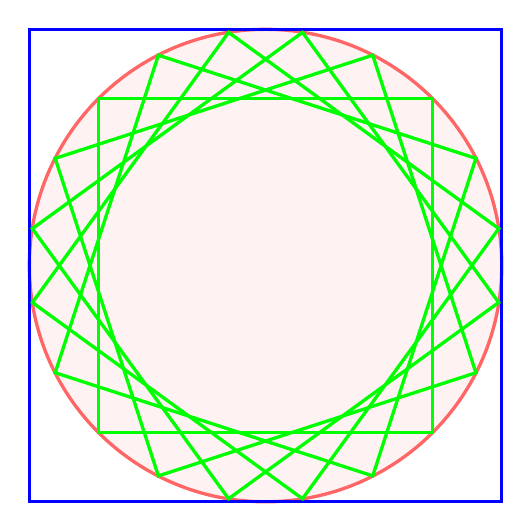
\begin{tikzpicture}[scale=2.]
		\filldraw[color=red!60, fill=red!5, very thick](0,0) circle (1.5);
		\draw[blue, very thick] (-1.5,-1.5) rectangle (1.5,1.5);
		\draw[green, very thick, rotate around={0:(0,0)}](-1.06,-1.06) rectangle (1.06,1.06);
		\draw[green, very thick, rotate around={72:(0,0)}](-1.06,-1.06) rectangle (1.06,1.06);
		\draw[green, very thick, rotate around={144:(0,0)}](-1.06,-1.06) rectangle (1.06,1.06);
		\draw[green, very thick, rotate around={216:(0,0)}](-1.06,-1.06) rectangle (1.06,1.06);
		\draw[green, very thick, rotate around={288:(0,0)}](-1.06,-1.06) rectangle (1.06,1.06);
		\end{tikzpicture}
	
		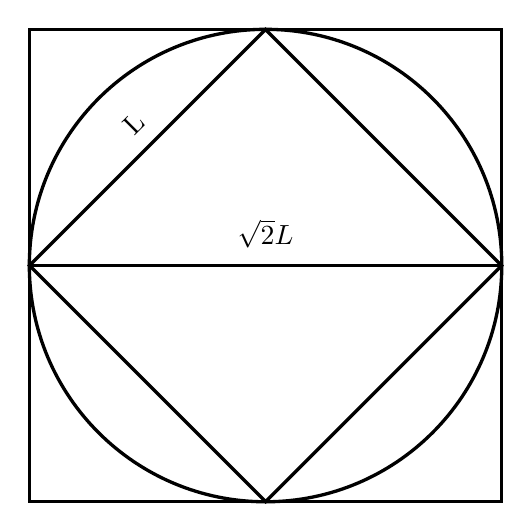
\begin{tikzpicture}[scale=2.]
		\draw[black, very thick] (-1.5,-1.5) rectangle (1.5,1.5);
		\draw[black, very thick] (0, 0) circle (1.5);
		\draw[black, very thick, rotate around={45:(0,0)}](-1.06,-1.06) rectangle (1.06,1.06);
		\draw[black, very thick] (1.5,0.0) -- (-1.5,0.0);
		\draw (0.0,0.2) node {$\sqrt{2} L$};
		\node[label={[label distance=0.2,text depth=-1ex,rotate=45]L}] at (-0.75,0.75) {};
		\end{tikzpicture}
	\end{tabular}{cc}
\end{center}

%----------------------------------------------------------------------------------------
%	RESULTS 
%----------------------------------------------------------------------------------------

\section*{Results}

In table \ref{table-results} are shown the best results obtained from the use of different input sizes.

\begin{center}
	\captionof{table}{Best classification results achieved with one eye and two eyes information}	
	\begin{tabular}{*8c} 
		\hline
		&            & \multicolumn{3}{c}{One eye information} & \multicolumn{3}{c}{Two eyes information} \\
		Layers & Input size & $\kappa_{test}$ & FN & FP & $\kappa_{test}$ & FN & FP \\ [0.5ex] 
		\hline\hline
		12 & (3,128,128) & 0.488 & 11.6\%& 11.5\% & 0.555 & 11.2\%& 12.9\%\\ 
		14 & (3,256,256) & 0.636 & 4.4\%& 28.7\% & 0.661 & 4.4\% & 28.7\% \\ 
		16 & (3,384,384) & 0.668 & 7.9\%& 14.9\% & 0.722 & 11.2\% & 4.0\%  \\ 
		16 & (3,512,512) & 0.725 & 5.0\%& 11.9\% & 0.752 & 6.5\% & 7.0\% \\ 
		\hline
	\end{tabular}
	\label{table-results}
\end{center}

In table \ref{table:best-nn} we show the architecture of the best performing network.

\begin{center}
	\captionof{table}{Best performing architecture}
	\begin{tabular}{c c c c} 
		\hline
		Layer & Type & Characteristics & Output Size \\ [0.5ex] 
		\hline\hline
		0 & Input & 3 RGB channels & (3,512,512) \\ 
		1 & Conv & 8 fil 3x3 1,1 str, 1,1 pad & (8,512,512) \\
		2 & Conv & 16 fil 3x3 1,1 str, 1,1 pad & (16,512,512) \\
		3 & Conv & 16 fil 3x3 1,1 str, 1,1 pad & (16,512,512) \\
		- & Maxpool & 2,2 size, 2,2 str & (16,256,256) \\
		4 & Conv & 32 fil 3x3 1,1 str, 1,1 pad & (32,256,256) \\
		5 & Conv & 32 fil 3x3 1,1 str, 1,1 pad & (32,256,256) \\
		- & Maxpool & 2,2 size, 2,2 str & (32,128,128) \\
		6 & Conv & 64 fil 3x3 1,1 str, 1,1 pad & (64,128,128) \\
		7 & Conv & 64 fil 3x3 1,1 str, 1,1 pad & (64,128,128) \\
		- & Maxpool & 2,2 size, 2,2 str & (64,64,64) \\
		8 & Conv & 128 fil 3x3 1,1 str, 1,1 pad & (128,64,64) \\
		9 & Conv & 128 fil 3x3 1,1 str, 1,1 pad & (128,64,64) \\
		- & Maxpool & 2,2 size, 2,2 str & (128,32,32) \\
		10 & Conv & 128 fil 3x3 1,1 str, 1,1 pad & (128,32,32) \\
		11 & Conv & 128 fil 3x3 1,1 str, 1,1 pad & (128,32,32) \\
		- & Maxpool & 2,2 size, 2,2 str & (128,16,16) \\
		12 & Conv & 128 fil 3x3 1,1 str, 1,1 pad & (128,16,16) \\
		13 & Conv & 128 fil 3x3 1,1 str, 1,1 pad & (128,16,16) \\
		- & Maxpool & 2,2 size, 2,2 str & (128,8,8) \\
		14 & Conv & 256 fil 8x8 1,1 str, 1,1 pad & (256,8,8) \\
		15 & Fully connected & 256 elem & (256) \\ [1ex] 
		16 & Softmax & 256 to 5 elem & 5 \\ [1ex] 
		\hline
	\end{tabular}

	\label{table:best-nn}
\end{center}

%----------------------------------------------------------------------------------------
%	CONCLUSIONS
%----------------------------------------------------------------------------------------

\color{SaddleBrown} % SaddleBrown color for the conclusions to make them stand out

\section*{Conclusions}

In this paper is shown that deep learning techniques are a promising technique for solving medical imaging problems like the diabetic retinopathy detection. Having enough data this method is able to perform near human level expertise achieving $\kappa$ values of 0.752 not far from the $\kappa$ achieved by human experts, around 0.80. 

\color{DarkSlateGray} % Set the color back to DarkSlateGray for the rest of the content

%----------------------------------------------------------------------------------------
%	FORTHCOMING RESEARCH
%----------------------------------------------------------------------------------------

\section*{Forthcoming Research}

Future work will be centered on testing higher resolution input images, newer schemes such as residual networks, the use of alternative cost functions that encode the prior information of the ordering of the classes and more elaborated methods for combining the information coming from both eyes.

 %----------------------------------------------------------------------------------------
%	REFERENCES
%----------------------------------------------------------------------------------------

%\nocite{*} % Print all references regardless of whether they were cited in the poster or not
\bibliographystyle{unsrt} % Plain referencing style
\bibliography{retinopathy} % Use the example bibliography file sample.bib

%----------------------------------------------------------------------------------------
%	ACKNOWLEDGEMENTS
%----------------------------------------------------------------------------------------

\section*{Acknowledgements}

\small{This work is supported by the URV grant 2014PFR-URV-B2-60 and the Spanish research projects PI15/01150 and PI12/01535 (Instituto de Salud Carlos III). The authors would like to thank to the California Healthcare Foundation and EyePACS for providing the images used in this study.}

%----------------------------------------------------------------------------------------

\end{multicols}
\end{document}